\capitulo{5}{Aspectos relevantes del desarrollo del proyecto}

El desarrollo de este trabajo se ha estructurado en varias partes.
Por un lado, el desarrollo de la aplicación web que tiene que interactuar con el visitante del museo y el guía remoto. Por otro lado, también se ha desarrollado la API encargada de interconectar ambos elementos.
Además, con el fin de mejorar tanto la organización de las visitas guiadas como la experiencia del visitante, también se ha implementado un sistema de geolocalización \textit{indoor} basado en tecnología \textit{UWB}.
Por último, en este trabajo también se ha participado en parte del desarrollo del dibujado sobre obras de arte por parte del guía para su representación gráfica en el usuario, siendo este uno de los puntos claves para la realidad aumentada del proyecto.
\begin{comment}

Este apartado pretende recoger los aspectos más interesantes del desarrollo del proyecto, comentados por los autores del mismo.
Debe incluir desde la exposición del ciclo de vida utilizado, hasta los detalles de mayor relevancia de las fases de análisis, diseño e implementación.
Se busca que no sea una mera operación de copiar y pegar diagramas y extractos del código fuente, sino que realmente se justifiquen los caminos de solución que se han tomado, especialmente aquellos que no sean triviales.
Puede ser el lugar más adecuado para documentar los aspectos más interesantes del diseño y de la implementación, con un mayor hincapié en aspectos tales como el tipo de arquitectura elegido, los índices de las tablas de la base de datos, normalización y desnormalización, distribución en ficheros3, reglas de negocio dentro de las bases de datos (EDVHV GH GDWRV DFWLYDV), aspectos de desarrollo relacionados con el WWW...
Este apartado, debe convertirse en el resumen de la experiencia práctica del proyecto, y por sí mismo justifica que la memoria se convierta en un documento útil, fuente de referencia para los autores, los tutores y futuros alumnos.
- Base de datos
- Uso de React
- Uso de Enpoints
- Uso de Raspberrys
- Uso de OpenAPI
- Uso de Arquitectura pasiva para la triangulación
\end{comment}

\section{Desarrollo de la aplicación web}
Para el desarrollo de la aplicación web había que tener en cuenta la presencia de dos tipos de usuario, visitante del museo y guía remoto. Por el lado del visitante tendríamos el inicio de sesión en el sistema para recibir el vídeo y el audio del guía, y por el lado del guía tendríamos que insertar la geolocalización de cada visitante en su sala y el \textit{canvas} para poder dibujar sobre las imágenes recibidas desde los visitantes.

Durante el desarrollo de la aplicación surgieron diferentes momentos en los que se tuvieron que tomar distintas decisiones sobre cómo desarrollar el software o qué tecnología utilizar, sobre todo en la fase de investigación.

Dado que la interfaz del guía debe incluir la localización de los visitantes, en las primeras fases del proyecto surgieron distintas soluciones para decidir qué librería de mapas se podría utilizar:

\begin{itemize}
    \item \textbf{Carto}. Es un software de bases de datos de alto rendimiento para integración de mapas, compatible con implementaciones de distintos tipos de servicios de localización a tiempo real. La desventaja es que el software de su API web proporcionado es de pago y no es código abierto en su totalidad.
    \item \textbf{Leaflet} - Usando mapa de \textit{OpenStreetMap}. Librería para el desarrollo de mapas en diferentes entornos. En este proyecto en particular se tuvo en cuenta su librería de \textit{javascript}, es de código abierto, pero no cuenta con muchas funcionalidades para la interacción con los usuarios.
    \item \textbf{OpenLayers}. Es otra librería para el desarrollo de mapas, normalmente en entornos web. Se utilizó su versión de \textit{javascript}, debido a que su código era abierto y es una de las librería de mapas más completas que existen a día de hoy para la interacción con los usuarios. 
    \item \textbf{Google Indoor Location}. Solución software de Google para mostrar usuarios en interiores. Se descartó esta solución debido a que solo permitía el uso de la API de mapas de Google.
    \item \textbf{MapWize}. Solución para mostrar usuarios en entornos \textit{indoor}. Se descartó por ser de pago y ya tener un prototipo con herramientas \textit{open source}.
\end{itemize}

Se tenía pensado desde un principio que \textit{React} iba a ser la librería a utilizar,
debido a que se contaba con experiencia previa desarrollando con este \textit{framework} y 
así agilizaría todo a la hora de crear código para el entorno web.

Se creó un proyecto por separado de \textit{OpenLayers} en \textit{Javascript Vainilla} a modo de prueba de concepto para poder implementar una versión básica del mapa, para poder entender los conceptos de cómo funcionan los mapas en la librería y cómo implementarlos con \textit{Javascript}.

En la figura 5.1 se puede ver una implementación de un mapa con \textit{OpenLayers} donde se muestra un \textit{Tag} en azul, un \textit{Anchor} con un cuadrado rojo, que indica que ha sido movido y no guardado en la base de datos, y dos \textit{Rooms}.
\begin{figure}[t]
    \centering
    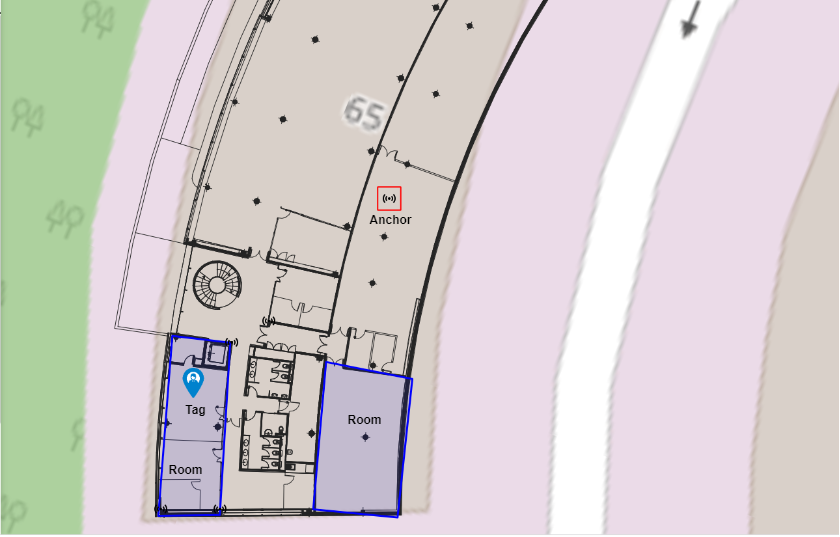
\includegraphics[width=10cm,height=10cm,keepaspectratio]{img/OpenLayers.png}
    \caption{Mapa con OpenLayers con un Tag, dos Rooms y un Anchor con bordeado rojo.}
    \label{fig:Example OpenLayers}
\end{figure}

Llegó un reto importante que era exportar como una capa los planos del edificio donde se iban a realizar las pruebas de despliegue, que en este caso iban a ser las oficinas de Vicomtech. Para realizar este procedimiento se utilizó un software especifico de mapas llamado \textit{QGIS}, el cual fue bastante complejo de entender debido a que está orientado a arquitectos y topógrafos profesionales, por lo que utilizaba terminología desconocida hasta el momento.

Para la exportación de los planos, se importó de un proyecto Autocad como una capa y otra capa sería el mapa en sí. Una vez se tuvieron las capas juntas se procedió a colocar la capa de la estructura en la posición dónde se necesitara, cambiando el centro de coordenadas y el formato de exportación del mapa a \textit{EPSG:3857}, compatible con la librería. 

En la figura 5.2 se puede ver la base del edificio superpuesto como capa en el mapa.

\begin{figure}[t]
    \centering
    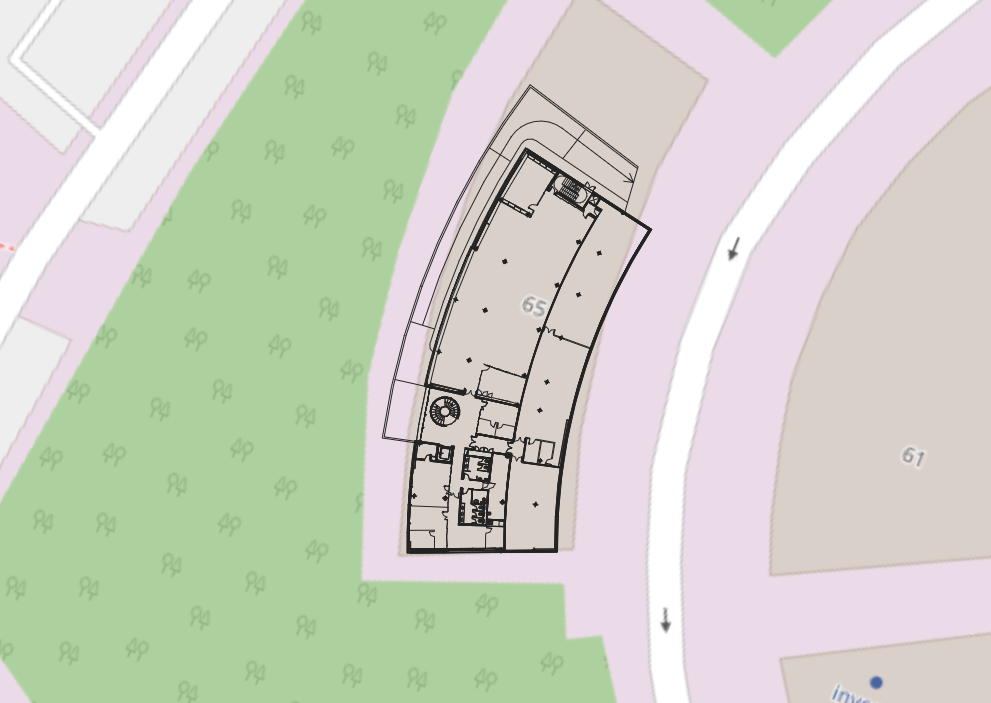
\includegraphics[width=10cm,height=10cm,keepaspectratio]{img/Base Edificio.png}
    \caption{Base de edificio en mapa con \textit{OpenLayers}.}
    \label{fig:Example OpenLayers}
\end{figure}
Una vez en este punto se utilizó un \textit{plugin} del propio \textit{software} que exportaba el proyecto \textit{QGIS} en una web estática con los siguientes elementos:

\begin{itemize}
    \item \textit{HTML} con las etiquetas necesarias para la inicialización del mapa.
    \item \textit{CSS} con los estilos básicos para la visualización del mapa.
    \item \textit{Javascript} con la importación de \textit{OpenLayers} y todo el uso de las funciones de la librería para la creación de capas e inicialización del mapa en la etiqueta asignada.
\end{itemize}

La creación de la capa de los planos se hacía mediante la exportación de la capa a un \textit{JSON} en formato \textit{EPSG:3857} Mismo formato que el mapa, esto se desarrolló en el proyecto estático donde ya existía una implementación de la librería con algunas interacciones referentes al mapa programadas previamente.

Tras esto tocó adaptar la librería \textit{OpenLayers} a \textit{ReactJs}, ya que no existía ninguna que adaptara \textit{OpenLayers} \textit{(Javascript Vainilla)} a componentes \textit{React}. Esto llevó un tiempo considerable, ya que tocó reescribir las funciones de inicializado de mapas en un componente \textit{React}, combinando la sintaxis de los componentes con la sintaxis de \textit{Javascript} puro.

Una vez existía interacción entre la aplicación \textit{React} y la \textit{API} tocó implementar distintas funcionalidades que mejoraran la experiencia de usuario cómo:

\begin{itemize}
    \item Mostrar a los \textit{Anchors} en el mapa, poderlos mover, y que se pueda persistir la nueva posición. También se añadió un bordeado rojo para aquellos \textit{Anchors} que se muevan y no se guarden.
    \item Mostrar a los \textit{Tags} ligados a usuarios en el mapa, en base a la posición de las coordenadas de la base de datos.
    \item Mostrar \textit{Rooms} existentes en la base de datos como un polígono. También se añadió una página para poder eliminar y añadir \textit{Rooms} dibujando en el mapa.
\end{itemize}

Para mejorar la experiencia de usuario se implementaron unas restricciones en el \textit{login} de los usuarios normales, para comprobar que el usuario no estaba ligado ya a esa sesión o que estaba siendo usado.

Posteriormente a esto, y como último paso, se implementó una función que comprobara el estado de los \textit{tags} con usuarios en la base de datos, y que de manera dinámica identificara qué capas hacía falta borrar, actualizar o añadir en base a la información recibida a 1 Hz, coincidiendo con el la frecuencia de actualización de los Raspberries en la base de datos.

Después se implementó un sistema de dibujado mediante sobreposición de \textit{canvas}, colocando un \textit{canvas} con la obra de arte en el fondo y el \textit{canvas} de dibujado encima, así conseguimos que se pueda dibujar en la obra de arte. Ejemplo de esto se muestra en la figura 5.3.

\FloatBarrier
\begin{figure}[h]
    \centering
    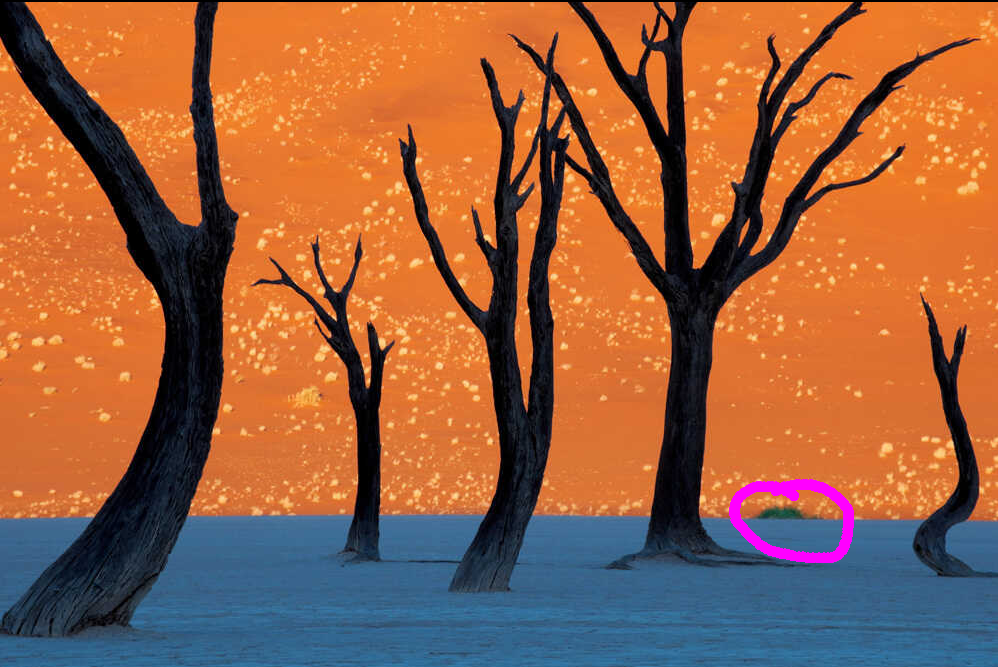
\includegraphics[width=10cm,height=10cm,keepaspectratio]{img/P5Example.png}
    \caption{Dibujado en dos capas con librería \textit{P5}.}
    \label{fig:Example-P5}
\end{figure}
\FloatBarrier
\section{Desarrollo de la API}
Para el desarrollo de la \textit{API} se ha utilizado el estándar \textit{OpenAPI}. Esto permitió utilizar la herramienta \textit{Swagger Editor} (figura 5.4) para escribir las especificaciones necesarias en base a un documento con extensión \textit{yaml}. Este incluye tanto el diseño de los casos de uso como el diseño de los \textit{endpoints} que se iban a utilizar. Esta herramienta permitió poder auto generar una versión de la \textit{API} con \textit{Python} y \textit{Flask}, todo implementado con \textit{docker}.

\begin{figure}[t]
    \centering
    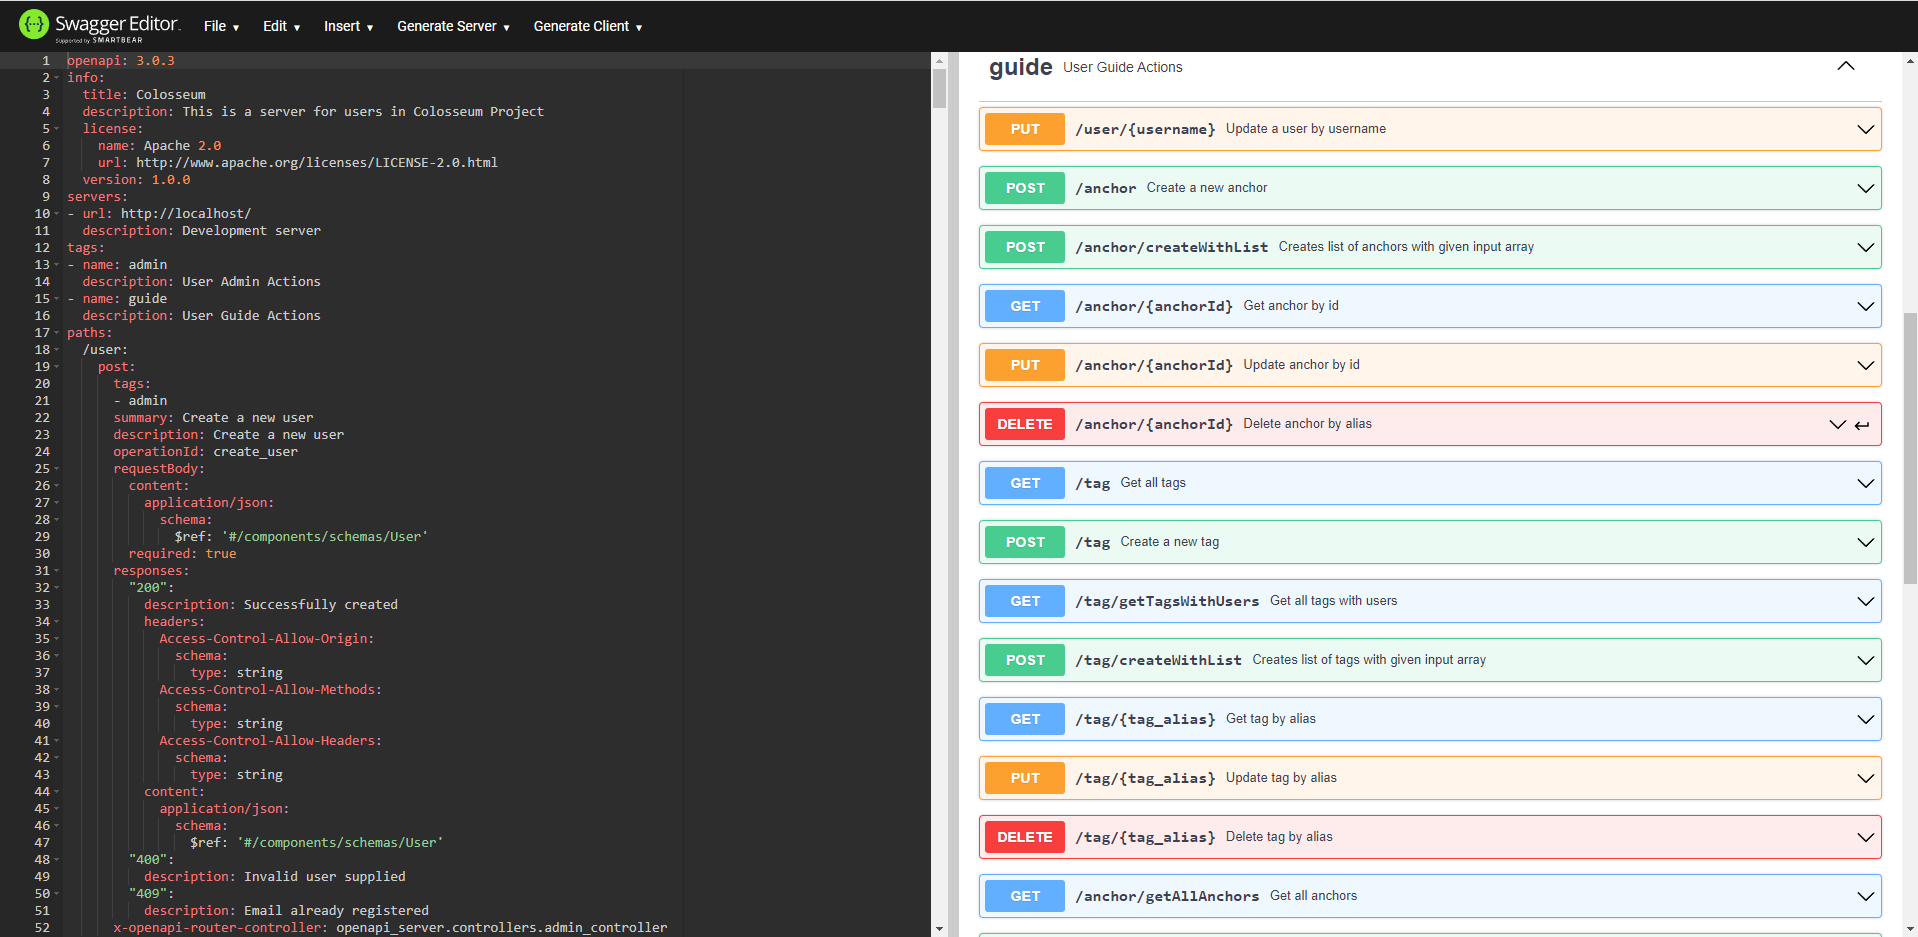
\includegraphics[width=10cm,height=10cm,keepaspectratio]{img/SwaggerEditor.png}
    \caption{Herramienta web \textit{Swagger Editor} con las especificaciones de la \textit{API}.}
    \label{fig:Swagger Editor}
\end{figure}
A esta primera versión auto generada se le tuvo que añadir la librería \textit{Connexion}, para poder generar acceso a los \textit{endpoints} por HTTP en base a la especificación del documento \textit{yaml}.

Para la conexión con la base de datos se añadió:
\begin{itemize}
    \item \textit{\textbf{SqlAlchemy}}, para la gestión de la base de datos a modo de objetos en\textit{Python}.
    \item \textit{\textbf{Marshmellow}}, librería que funciona a modo de \textit{wrapper} necesaria para el funcionamiento de \textit{SqlAlchemy}.
\end{itemize}

Una vez llegados a este punto se tuvo en cuenta la posibilidad de implementar bases de datos óptimas para operaciones con mapas como:
\begin{itemize}
    \item \textit{\textbf{CartoDB}}, una implementación de una base de datos de alto rendimiento basada en \textit{Redis} e implementada por la empresa \textit{Carto}.
    \item \textit{\textbf{MySQL}} como instancia con \textit{Docker}. Al necesitar crear distintas tablas personalizadas para la aplicación, esta opción fue la más flexible para realizar el desarrollo, ya que todo el proyecto se encapsuló en \textit{Docker} para poder automatizar el despliegue y eso lo hizo más compatible con el \textit{ORM SQLAlchemy}.
\end{itemize}

Finalmente se acabó utilizando una instancia \textit{MySQL} en \textit{Docker}  previamente configurada, lo que permitió hacer una conexión rápida a través del \textit{ORM} en la \textit{API}.

Una vez tuvimos todo configurado y conectado, se pasó a realizar la lógica en la parte de los controladores, manejando todas las instrucciones que interactúan con la base de datos que van a ser recibidos por peticiones \textit{HTTP}, e incluso manejando la lógica independiente para añadir, modificar, consultar, eliminar o intersectar objetos en las funcionalidades de \textit{geofencing} \textit{Tile38} utilizando su librería cliente \textit{pyle38}.

\section{Despliegue}
Para el despliegue de la aplicación  web se utilizó una instancia de \textit{Docker} de \textit{Nginx} previamente configurada. Esto permitió un despliegue de la aplicación web a producción de manera que fuese lo más rápido y óptimo posible. Para esto, en vez de utilizar el servidor \textit{HTTP} que compila el código escrito en \textit{react} llamado \textit{react-scripts}, utilizamos \textit{Vite}, que era similar en funcionalidades pero mucho mas rápido, reduciendo así los tiempos para el despliegue y compilación de la aplicación.


\section{Sistema de geolocalización \textit{indoor}}

En las primeras etapas del proyecto se tuvo que analizar qué tipo de tecnología que se iba a utilizar para la geolocalización teniendo en cuenta parámetros como
la latencia de la comunicación, la frecuencia aproximada a la que trabajan los dispositivos de las distintas tecnologías o la resistencia ante interferencias que tengan los dispositivos seleccionados para la fiabilidad de los datos.

Finalmente se consideró utilizar placas \textit{Ultra Wide Band} debido a que en un futuro no muy lejano, gran parte de los teléfonos inteligentes tendrán un \textit{chip} UWB incluido, lo que hace que sea una tecnología muy prometedora.

Para toda la implementación de sistema de geolocalización se utilizaron placas \textit{MDEK1001 UWB} a las que se le cambió el \textit{firmware}, debido a que necesitábamos tener los \textit{anchors} como dispositivos pasivos que reciben y responden comunicaciones, los \textit{tags} para comenzar las comunicaciones, y otras placas actuando como \textit{listener} para comunicarnos con la \textit{raspberry}. Estos roles permitieron crear una arquitectura de placas pasivas-activas, donde la placa o \textit{tag} activa se comunica con los dispositivos pasivos para triangular su posición en el sistema de representación local.

Una vez que se conoce su representación local de las \textit{tag}, se comunican con la placa que hace de \textit{listener}. Esta placa hace de intermediaria entre la \textit{raspberry} y las \textit{tags}, y su función consiste en recibir las posiciones de las placas \textit{tag} y enviárselas a la \textit{raspberry}.

Tras la recepción de las posiciones en la \textit{raspberry}, su función ahora es filtrar \textit{tags} para no obtener duplicados, y hacer la traslación de coordenadas de la representación local a la representación compatible para su representación en el mapa.


En las \textit{Raspberries} al principio se implementó un \textit{firmware} de \textit{FIND3}, que hace de servidor unificando los datos de las conexiones de los \textit{tags UWB}. Crea un servicio web en el que se pueden ver estadísticas e incluso puede utilizar modelos entrenados para hacer \textit{geofencing}. Además \textit{FIND3} cuenta con una \textit{api} para que puedas interactuar con el servicio. Finalmente se implementó un software desde cero debido a que \textit{FIND3} no tenía la precisión necesaria que requería el proyecto.


Las placas \textit{MDEK1001} elegidas pueden ser consultadas mediante una \textit{app} para \textit{Android} vía \textit{Bluetooth Low Energy (BLE)}, permitiendo así modificar su configuración  y ver su ubicación local en una interfaz gráfica.

En la figura 5.5 se puede ver una imagen de un sistema de placas \textit{UWB} donde un \textit{Tag}, representado con un círculo morado, triangula de manera activa su posición en la representación local, en función de los \textit{Anchors}, representados como triángulos rojos, que actúan de manera pasiva.

\begin{figure}[t]
    \centering
    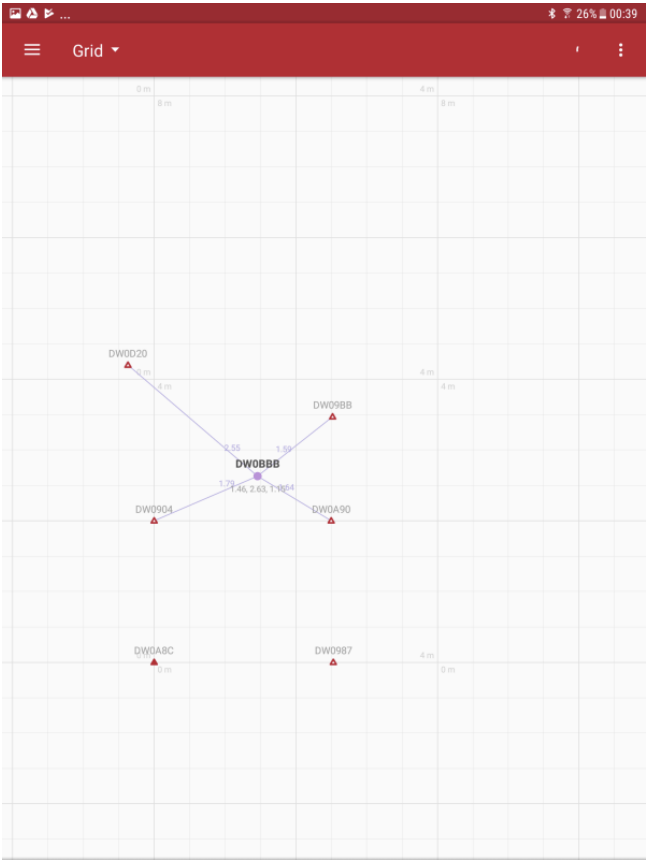
\includegraphics[width=10cm,height=10cm,keepaspectratio]{img/LocationTags.png}
    \caption{Aplicación del fabricante donde se muestra la ubicación local de un \textit{tag}.}
    \label{fig:app-local-representation}
\end{figure}



\section{Pruebas}
Las pruebas de la aplicación se han basado en el rendimiento de las placas en diferentes entornos realistas y su representación en el mapa en tiempo real. 

Los casos probados fueron:
\begin{itemize}
    \item Una sala con 3 \textit{Anchors}, un 1 \textit{Tag}, 1 \textit{Listener} y 1 \textit{Raspberry} para su triangulación y diferentes cuadros colgados en la habitación para probar la realidad aumentada creada para las visitas del guía.
    \item Dos sala con 3 \textit{Anchors} cada una, un 1 \textit{Tag}, 2 \textit{Listener} y 2 \textit{Raspberry} para su triangulación y diferentes cuadros colgados en la habitación para probar la realidad aumentada creada para las visitas del guía.
    \item Una sala con 3 \textit{Anchors}, un 3 \textit{Tags}, 1 \textit{Listener} y 1 \textit{Raspberry} para su triangulación y diferentes cuadros colgados en la habitación para probar la realidad aumentada creada para las visitas del guía.
    \item Dos sala con 3 \textit{Anchors} cada una, un 4 \textit{Tag}, 2 \textit{Listener} y 2 \textit{Raspberry} para su triangulación y diferentes cuadros colgados en la habitación para probar la realidad aumentada creada para las visitas del guía.
\end{itemize}

En la figura 5.6 se muestra el tercer caso de prueba donde existen 3 \textit{Tags}, 3 \textit{Anchors} y 1 \textit{Listener} en una sala física, con el esquema de flujo de de datos. Siendo la prueba más compleja de una sala.

\begin{figure}[t]
    \centering
    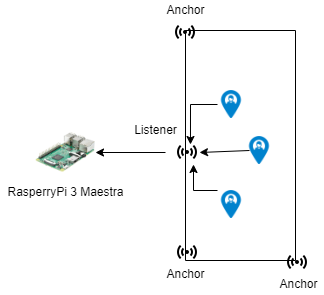
\includegraphics[width=10cm,height=10cm,keepaspectratio]{img/Esquema de coenxiones.png}
    \caption{Caso de prueba de 3 \textit{Tags}, 3 \textit{Anchors} y 1 \textit{Listener} en una sala.}
    \label{fig:app-local-representation}
\end{figure}
Los resultados fueron bastante satisfactorios llegando a una precisión de 20 cm, lo cual supera el objetivo de investigación de 50 cm de precisión en la horizontal. Al no tener diferentes plantas, finalmente no se tuvo en cuenta la precisión vertical.

También se realizó una prueba de estrés, con un script en \textit{Python}, del mapa añadiendo tags simulados a la base de datos, generando una longitud y latitud aleatorias en un rango determinado, para poder ver la frecuencia de actualización en el mapa y cuánto era límite máximo de frecuencia que permitía el mapa. En este caso los resultados fueron muy satisfactorios ya que el objetivo era trabajar insertando 1 \textit{tag} por segundo, y los resultados llegaron a 3 \textit{tags} por segundo, teniendo margen suficiente para interactuar con otras partes del sistema.